The ingredients are composed of basic object reconstruction, tracks and clusters.
The reconstruction of chared particle tracks are made using hits on sensitive layers from either tracker system or the muon detector.
The interation points of proton-proton collisions can be build using the positions of reconstructed vertices associated with the reconstructed tracks.
Another basic object, the clusters, can be built using the dedicated clustering algorithm with the position and energy deposited of electromagnetic and hadronic showers from ECAL and HCAL.
\subsection{Track}
The tracks left in the tracking system by charged particles are in a helix structure with 5 degree of freedom: 3 from the particle velocity, 3 from the particle initial position, and -1 from the helix constrain.
The individual hits on the detectors are fitted to an expected track of a particle during the reconstruction.
The sensor elements are triggered when the particles pass the detector modules at certain angle, and the clusters of neighboring sensor elements are joined together as hits.

The weighted average of sensor component coordinates in a cluster can determine the spacial position of hits, which would be further corrected with the incidence angle and corresponding energy deposits when the track is reconstructed.
A dedicated tracking software called the combinatorial track finding (CTF) algorithm which runs several iterations of combinatorial Kalman filter~\cite{Fruhwirth:1987fm} integrating patter recognition and track fitting.
Each tracking iteration is composed of four steps: track seeding, trajectory building, ambiguity resolving, and track fitting~\cite{CMS:2014pgm}.
Figure~\ref{fig:reco_track} shows the tracking efficiency achieves $98\%$ in the CMS experiment.

\begin{figure}\centering
    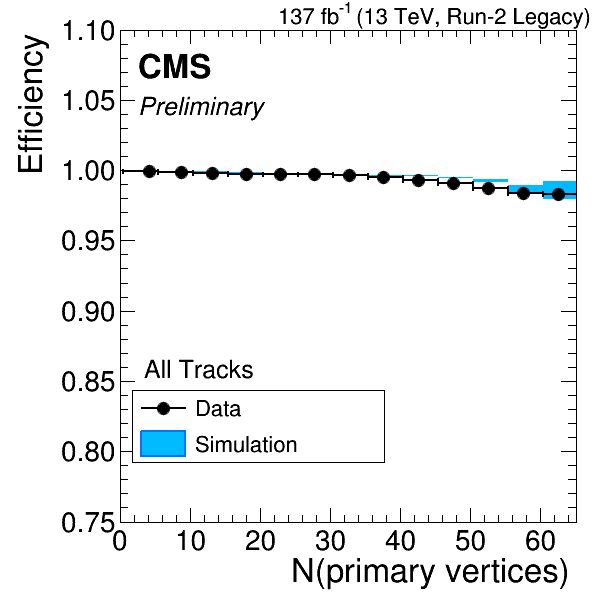
\includegraphics[width=0.5\textwidth]{figure/reco_track.png}
    \caption[The tracking efficiency as a function of the number of primary vertices in the all tracks collection.]
    {
        The tracking efficiency as a function of the number of primary vertices in the all tracks collection. 
        Data (black dots) and \MADGRAPH DY (light blue rectangles). 
        The uncertainties shown are statistical.
    }
    \label{fig:reco_track}
\end{figure}

\textbf{Track seeding} sets the initial trajectory parameters and their uncertainties in the beginning of the reconstruction of a track.
Iconic signatures, for example, the good hits in the pixel detector with close spacial proximity and orientation towards the interaction point are used in the first iterations to give a good estimation of the particle track.
Looser criteria are used in the following iterations to ensure particles decaying in flight in the tracking system is also reconstructed

\textbf{Trajectory building} is commonly referred as the KF process, updating the trajectory parameters at each layer.
It is done by propagating the existing trajectory to the next layer, choosing a hit within a certain neighborhood, and correcting the trajectory parameters from a $\chi^2$ fit.
Multiple additional trajectory candidates are generated when multiple candidate hits exist.
An invalid hit can be an additional information if a particle passes through a detector module without leaving any readout signal, and can be added into the list of hits in the trajectory candidate to indicate where a hit was expected to be.
The procedure is repeated layer by layer until termination conditions, such as poor fitting results (large $\chi^2$, low expected \PT), need for speeding up computations (terminate after finding some consecutive hits), or large number of consecutive invalid hits. 
The hits associated with track candidates can be masked from the list after the first iteration of the trajectory building algorithm.
The process can then restart with a new set of track seeds made with looser seeding criteria.
The CMS performs 5 iterations of the track building with progressively looser criteria for seeding in each iteration for the standard track reconstruction.
This allows particles originating from in-flight decays with as little as 3 hits be constructed.

\textbf{Ambiguity resolving} is then needed to avoid track double counting caused by the multiple trajectory candidates created at each propagation in the trajectory building algorithm.
The track with the larger $\chi^2$ values will be discarded as a duplicate between two track candidate with the fraction of shared hits is greater than $50\%$.

\textbf{Track fitting} reruns the track fitting on the hits among track candidates to reduce biases introduced by the seed selections, and also update the hit information with now-available track information.

\subsection{Vertex}
Vertexing algorithm plays an important role in indicating the physics interaction point by finding the point where trajectories meet.
Primary vertexes close to the beam line and the desired interaction point are expected to be the reconstructed coordinate with large numbers of associated tracks.
Secondary vertexes, in contrast, are points of particles decaying in-flight and expected to have significantly smaller number of associated tracks and a larger transverse distance from the beam line.
Secondary vertexes are collected with subsets of tracks associated with physical objects, and are typically reconstructed only after the primary vertex has been reconstructed.

The results of a $\chi^2$ fit of a vertex position can be done by minimizing a function of sum of standardized distance squared $L(\vec{v})$ as:
\begin{linenomath}\begin{equation}\label{eq:reco_fit}
    L(\vec{v}) = \frac{1}{2} \sum_i \chi^2(\vec{v}, \vec{x_i}) = \sum_i \Bigl( \frac{d_i(\vec{v})}{\sigma_i} \Bigr)^2
\end{equation}\end{linenomath}
where $i$ runs over the indexes of tracks, $d_i(\vec{v})$ is the distance of the vertex position from track $i$, and $\sigma_i$ is the uncertainty in the distance.
However, poorly associated tracks contribute large $\chi^2$ values in this method.
The adaptive vertex fitter~\cite{Fruhwirth:2007hz} sequentially suppresses potentially outlying tacks instead by an additional weighting function:
\begin{linenomath}\begin{equation}\label{eq:reco_weight}
    w(\chi^2) = \frac{\mathrm{exp}(-\chi^2/2T)}{\mathrm{exp}(-\chi^2/2T)+\mathrm{exp}(-\chi^2_c/2T)}
\end{equation}\end{linenomath}
where $T$ is a temperature variable indicating how sensitive the minimization is with large $\chi^2$, and $\chi_C$ is a constant for which $w(\chi_C)=1/2$.
The minimization of Eq.~\ref{eq:reco_fit} can be solved with the weight applied as 
\begin{linenomath}\begin{equation}\label{eq:reco_temp}
    \sum_i w(\chi_i(\vec{x}))\chi(\vec{v})\frac{\partial\chi(\vec{v})}{\partial\vec{v}} = 0.
\end{equation}\end{linenomath}

Then, solve Eq.~\ref{eq:reco_temp} using some augmented function $F(\vec{v})$ instead of $L(\vec{x})$ with the effective $\chi^2$ noted as $\rho(x)$ is give associated
\begin{linenomath}\begin{equation}\label{eq:reco_rho}
    \rho(x) = \frac{1}{2}\chi^2 - Tln\biggl( \frac{1+\mathrm{exp}(\chi^2_C / 2T)}{\mathrm{exp}(\chi^2/2T)+\mathrm{exp}(\chi^2_C/2T)}\biggr).
\end{equation}\end{linenomath}
In the limit of $T\rightarrow 0$, $\rho(\vec{v})$ approaches the original $\chi^2/2$ for $\chi < \chi_C$ and a fixed value for $\chi > \chi_C$ as shown in Fig.~\ref{fig:reco_vertex}.
The minimization of extreme outliers at small $T$ is then expected to be negligible.
The $\chi_C$ is set to 3 in the official operation for reconstructing the primary vertexes because the vertex only has 3 degrees of freedom.
\begin{figure}[H]\centering
    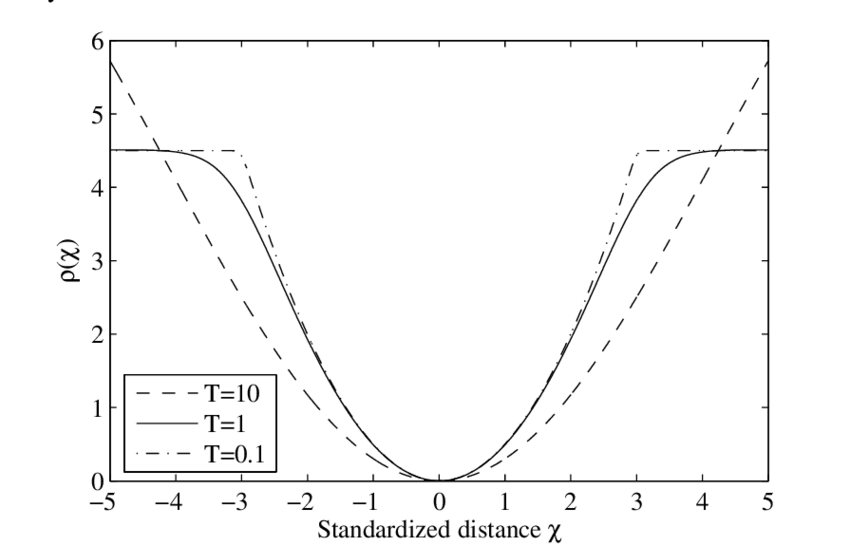
\includegraphics[width=0.5\textwidth]{figure/reco_vertex.png}
    \caption{
        Effective $\chi^2$ function $\rho(\chi)$ at various temperature parameters $T$.
    }
    \label{fig:reco_vertex}
\end{figure}


The initial point of the vertex fitting algorithm is determined by the algebraic mean of the closest point pairs of two tracks.
A weighting value $w=(d+d_{min})^{-1/2}$, where $d$ is the distance of minimal approach, and $d_{min}$ is an offset value of 10$\mu$m then determines the track pair with the largest $w$.
Tracks with small $\chi^2$ are seemed to be associated with the vertex after the vertex is reconstructed.
Tracks without any vertex associated are reiterated to reconstruct primary vertex.

\subsection{Calorimeter clustering}
Clustering algorithms are designed to identify individual particles coming from different physical interactions, while distinguish particles originating from interaction points from particles coming from soft radiation processes.
It is composed of two steps: cluster seeding and topological clustering.

Cluster seeding initialize the clustering algorithm with local maximums which is larger than the expected noise in the calorimeters.

Topological clustering joins particle-flow clusters with neighbor cells with an energy above a certain threshold (80 \MeV in the ECAL barrel, 300 \MeV in the ECAL endcap, and 800 \MeV in the HCAL).
The clustering algorithm has not yet resolved the ambiguity of cells associated with multiple particle-flow clusters at this step.
The cell ambiguity is resolved using the calorimeter granularity after all particle flow clusters has finished the topological clustering process.
